% !TeX spellcheck = en_GB

\documentclass[preprint,12pt]{elsarticle}
%% Use the option review to obtain double line spacing
%% \documentclass[preprint,review,12pt]{elsarticle}

\usepackage{lmodern}
\usepackage[utf8]{inputenc}
\usepackage[english]{babel}

%% Use the options 1p,twocolumn; 3p; 3p,twocolumn; 5p; or 5p,twocolumn
%% for a journal layout:
%% \documentclass[final,1p,times]{elsarticle}
%% \documentclass[final,1p,times,twocolumn]{elsarticle}
%% \documentclass[final,3p,times]{elsarticle}
%% \documentclass[final,3p,times,twocolumn]{elsarticle}
%% \documentclass[final,5p,times]{elsarticle}
%% \documentclass[final,5p,times,twocolumn]{elsarticle}

%% The graphicx package provides the includegraphics command.
\usepackage{graphicx}
\usepackage{amssymb}
\usepackage{amsmath,empheq, amsfonts}
\usepackage{subcaption}
\usepackage[section]{placeins}
\usepackage{mathtools}  

\usepackage{amsthm}
\newtheorem*{remark}{Remark}

%% The amsthm package provides extended theorem environments
%% \usepackage{amsthm}

%% The lineno packages adds line numbers. Start line numbering with
%% \begin{linenumbers}, end it with \end{linenumbers}. Or switch it on
%% for the whole article with \linenumbers after \end{frontmatter}.
\usepackage{lineno}

% Pseudocode
\usepackage{algorithm2e}
\SetKw{KwBy}{by}

%% natbib.sty is loaded by default. However, natbib options can be
%% provided with \biboptions{...} command. Following options are
%% valid:

%%   round  -  round parentheses are used (default)
%%   square -  square brackets are used   [option]
%%   curly  -  curly braces are used      {option}
%%   angle  -  angle brackets are used    <option>
%%   semicolon  -  multiple citations separated by semi-colon
%%   colon  - same as semicolon, an earlier confusion
%%   comma  -  separated by comma
%%   numbers-  selects numerical citations
%%   super  -  numerical citations as superscripts
%%   sort   -  sorts multiple citations according to order in ref. list
%%   sort&compress   -  like sort, but also compresses numerical citations
%%   compress - compresses without sorting
%%
%% \biboptions{comma,round}

% \biboptions{}

\journal{Neurocomputing}

\begin{document}
	
	\begin{frontmatter}
		
		%% Title, authors and addresses
		\title{RoS-LSSVM: Robust and Sparse Least Squares Support Vector Machines for Classification}
		%\title{Sparse, Robust Least Squares Support Vector Machines for the Classification of noisy datasets}
		
		%% use the tnoteref command within \title for footnotes;
		%% use the tnotetext command for the associated footnote;
		%% use the fnref command within \author or \address for footnotes;
		%% use the fntext command for the associated footnote;
		%% use the corref command within \author for corresponding author footnotes;
		%% use the cortext command for the associated footnote;
		%% use the ead command for the email address,
		%% and the form \ead[url] for the home page:
		%%
		%% \title{Title\tnoteref{label1}}
		%% \tnotetext[label1]{}
		%% \author{Name\corref{cor1}\fnref{label2}}
		%% \ead{email address}
		%% \ead[url]{home page}
		%% \fntext[label2]{}
		%% \cortext[cor1]{}
		%% \address{Address\fnref{label3}}
		%% \fntext[label3]{}
		
		
		%% use optional labels to link authors explicitly to addresses:
		
		
		\author[statistics]{Iwein Vranckx\corref{mycorrespondingauthor}}
		\cortext[mycorrespondingauthor]{Corresponding author}
		\ead[url]{wis.kuleuven.be/stat/robust}
		\ead[mail]{iwein.vranckx@kuleuven.be}
		
		\author[stadius]{Joachim Schreurs}
		\author[mebios]{Bart De Ketelaere}
		\author[statistics]{Mia Hubert}
		\author[stadius]{Johan Suykens}
		%
		\address[statistics]{KU Leuven, Department of Mathematics and LStat, Celestijnenlaan 200B, BE-3001 Heverlee, Belgium}
		\address[stadius]{KU Leuven, ESAT-STADIUS, Kasteelpark Arenberg 10, BE-3001 Heverlee, Belgium}
		\address[mebios]{KU Leuven, Division of Mechatronics, Biostatistics and Sensors, Kasteelpark Arenberg 30, BE-3001 Heverlee, Belgium}
		
		\begin{abstract}
			Least squares support vector machines (LS-SVM) are popular methods to solve classification problems. The LS-SVM is an SVM version which involves equality instead of inequality constraints and works with a least squares cost function.
			In this way, the solution follows from a linear system instead of a quadratic programming problem. However, compared to normal SVM's, support vector sparseness is lost and the classifiers efficiency is highly influenced by outliers. In this paper, we discuss a method which can overcome these two drawbacks. Robustness is achieved by the kernel concentration steps, which allow us to estimate a robust estimator of multivariate location and scatter in feature space. Afterwards, the robust LS-SVM is pruned by sampling diverse points out of a region of interest, close to the decision boundary.	Experiments show that the method is highly robust against trainingset contamination, where extreme spareness simultaneous achieved without diminishing the performance. 
			
		\end{abstract}
		
		\begin{keyword}
			Robust support vector machines\sep Non-linear outlier detection \sep Support vector pruning \sep Sparse LS-SVM 
		\end{keyword}
	\end{frontmatter}
	
	%\linenumbers
	
	%%%%%%%%%%%%%%%%%	Comment the following lines when the paper is finished
	%\tableofcontents
	\newpage
	
	%% main text
	\section{Introduction}
	
	Least-squares support vector machines (LS-SVM) are powerful methods for solving pattern recognition and regression problems~\cite{suykens2002least}. The LS-SVM maps data to a higher dimensional space in which one constructs an optimal separating hyperplane. It has been applied to many real-world problems such as optimal control~\cite{suykens2001optimal}, financial time series prediction~\cite{van2001financial}, system identification~\cite{goethals2005identification}, electrical load forecasting~\cite{espinoza2006fixed} and many others. However, the classifier model has two major disadvantages. First, it is (very) sensitive to outliers, as the underlying system of equations lacks robustness. This results in the orientation of the separating hyperplane in the direction of anomalies which, in turn, might cause a large amount of misclassifications. The second disadvantage is that its solution lacks sparseness, which hinders the application of LS-SVM models for real-time prediction. \\
	
	To reduce the influence of outliers, Suykens et al.~\cite{suykens2002weighted} proposed the weighted LS-SVM. By iteratively assigning small weights to outliers and retraining, the method diminishes the effect of extreme values. Another solution was proposed by Yang et al.~\cite{yang2014robust}, where a truncated loss function is used in the objective that is solved by a concave-convex procedure and the newton algorithm. A third solution is suggested by Debruyne et al.~\cite{debruyne2009robustified}, which proposes a weighted LS-SVM classification where weights are equal to the spatial rank with respect to the other feature vectors in the class.
	
	In comparison to the standard support vector machines (SVM), the LS-SVM only requires solving a linear system, but it lacks sparseness in the number of solution terms. To solve this problem, Suykens et al.~\cite{suykens2000sparse} propose a method that iteratively prunes the datapoints with lowest support values and retrains. Yang et al.~\cite{yang2014sparse} propose a one-step compressive pruning strategy to reduce the number of support vectors. Fixed-size LS-SVM sparsifies the LS-SVM by selecting important point or landmark points based on the quadratic Renyi Entropy criterion~\cite{suykens2002least}. However the landmark points are fixed in advance and don't take into account information of the classification itself, which could lead to sub-optimal results. This is in contrast to the sparse LS-SVM~\cite{suykens2000sparse}, which chooses observations based on the impact on the classification boundary. A comparison of different pruning methods can be found in~\cite{hoegaerts2004comparison}. \\
	
	In this paper, we focus on tackling both problems at once.
	Other methods are found in~\cite{chen2018sparse}, where a primal formulation of the LS-SVM with a truncated loss is introduced, sparseness is obtained by the Nystr\"{o}m approximation. A second method is the weighted LS-SVM of Suykens et al.~\cite{suykens2002weighted}. We propose a robust LS-SVM based on the minimum covariance determinant (MCD)~\cite{hubert2010minimum}, which is known to be a highly robust 	estimator of multivariate location and scatter. However, in contrast to the original formulation, the location and scatter is determined in feature space using the kernel trick, which enables the detection of non-linear outliers. Afterwards extreme sparsity is obtained by determinantal point processes (DPP)~\cite{kulesza2012determinantal} (or maximizing the quadratic Renyi entropy~\cite{suykens2002least}), which are capable of selecting diverse samples. To summarize, our main contributions consist off:
	\begin{enumerate}
		\item The development of a robust algorithm that is able to detect non-linear correlated outliers.
		\item The development of a new LS-SVM support vector selection strategy, based on entropy and determinantal point processes.
	\end{enumerate}
	The aggregation of both method's intermediate results yields our robust LS-SVM pruning methodology. \\ 
	
	The remainder of this paper is organized as follows. A brief overview of LS-SVM is given in section~\ref{sec:lssvm}. In section \ref{sec:proposed} we propose our classifier pruning strategy. The extensive simulation results of both theoretical and real, industrial datasets listed in section~\ref{sec:exp} confirm the robustness, prediction time speed-up and improved classifier efficiency of our proposed method. Finally, our main findings and suggestions for further research are summarized in the conclusion, section~\ref{sec:conc}. 
	
	
	\section{LS-SVM for classification}
	\label{sec:lssvm}
	The classifier goal is to learn a prediction model that assigns the correct label $y \in \{+1, -1\}$ to an unseen test sample. Restated more formally, we seek a classifier that fits an optimal hyperplane between the two classes, where the hyperplane maximizes the distance to the closest point(s) of either class. 
	%This margin $||w||^{-1}$ maximization leads directly to a classifier with good generalisation properties, i.e: it will result in good classification performance on (unseen) test data, for example compared with density based estimators. \\
	Given an $p$-variate trainingsset $x \in \mathbb{R}^p$ and the binary class label $y_i \in \{+1,-1\}$ for observation $x_i$ with index $i = 1,..,n$, the following constrained optimization must be solved to obtain the LS-SVM representation of the hyperplane margin $||w||^{-1}$ maximization:
	
	\begin{gather}
	\label{eq:costfunction}
	\mathrm{min} \  J(w,b,e_i) = \frac{1}{2} w^T w + \frac{\gamma}{2} \sum_{i=1}^{n} e_i^2 \\
	\label{eq:lsconstraint}
	\textrm{such that } y_i[w^T \varphi(x_i) + b] = 1-e_i, \enskip i = 1,..,n
	\end{gather}
	
	Here $w^T \varphi(x_i) + b$ is the hyperplane based decision function of the classifier with corresponding parameters $w$ and $b$, where the regularization parameter $\gamma$ is used to control the over/under-fitting trade-off. Finally,  $\varphi(.)$ is the transformation from input space $\mathbb{R}^p$ to the kernel feature space $\mathcal{H}$. 
	
	The specified constraint states that every given multivariate sample should lie on the correct side of hyperplane. Stated differently, the classifier should predict the class label of each sample correctly, where each observation $x_i$ has an corresponding error $e_i$ due to the constraint equality sign. This implies that a LS-SVM loses its support vector sparseness compared to ordinary SVM's. \\
	
	This constrained optimization problem is solved by the optimality conditions of its Lagrangian $\alpha$ as follows:
	\begin{equation}
	L(w,b,e;\alpha) = J(w,b,e) - \sum_{i=1}^{n} \alpha_i(y_i [ w^T \varphi(x_i) + b]-1 + e_i).
	\label{eq:lagrangian}
	\end{equation}
	%Here, $\alpha_i$ is the Lagrange multiplier whose value can be either positive or negative, which is also different from the standard SVM proposed by Vapnik. 
	As a direct consequence of the equality sign in the given constraint, the specified Lagrangian is now solvable trough a linear system of equations:
	\begin{align}
	\frac{\partial L}{\partial w} &= 0 \rightarrow w = \sum_{i=1}^{n} \alpha_i y_i \varphi(x_i) \\
	\frac{\partial L}{\partial b} &= 0 \rightarrow \sum_{i=1}^n \alpha_i y_i = 0 \\
	\frac{\partial L}{\partial e_i} &= 0 \rightarrow \alpha_i = \gamma e_i,  \enskip i = 1,..,n \\
	\frac{\partial L}{\partial \alpha_i} &= 0 \rightarrow y_i [w^T \varphi(x_i) + b ] = 1 - e_i, \enskip i = 1,..,n	
	\end{align}
	Combining the first and last equation and defining $\Omega{(i,j)}$ using the kernel trick for two observations with index $i$ and $j$ as:
	\begin{align}
	\Omega{(i,j)} &= y_i y_j \varphi(x_i)^T \varphi(x_j) \\
	&= y_i y_j K(x_i, x_j).
	\end{align}
	Common kernels are:
	\begin{align}
	\mathrm{Linear} \  \mathrm{kernel:} \ K(x,y) &= x^\mathrm{T}y \\
	\mathrm{Polynomial} \ \mathrm{kernel:} \ K(x,y) &= (\tau + x^\mathrm{T}y)^d \\
	\mathrm{RBF} \ \mathrm{kernel:} \ K(x,y) &= \mathrm{exp}\Big(-\frac{||x-y||_2^2}{\sigma^2}\Big) 
	\end{align}
	This results in the following set of linear equations, where the kernel matrix $K$ transforms observations to the kernel feature space $\mathcal{H}$.
	
	\begin{equation}
	\begin{bmatrix}
	0 & y^T \\
	y & \Omega + \gamma^{-1} \mathrm{I}
	\end{bmatrix}	
	\begin{bmatrix}
	b \\
	\alpha
	\end{bmatrix}
	=
	\begin{bmatrix}
	0 \\
	1
	\end{bmatrix},
	\end{equation}
	where $y  = [y_1;...;y_n]$, $1 = [1;...;1]$ and $\mathrm{I}$ the identity matrix.
	The least squares solution of the aforementioned system of equations is then used to  obtain the Lagrange coefficients $\alpha$ and offset $b$, where the decision function used for test set prediction is defined as:
	\begin{equation}
	\hat{y}(x) = \mathrm{sign}\Big(\sum_{i=1}^{n} \alpha_i y_i K(x, x_j) + b\Big).
	\label{eq:classification}
	\end{equation}
%	Or, written in a more convenient matrix notation, short-writing $\beta_i= (\alpha_i \  y_i)$
%	\begin{equation}
%	\hat{y}(x) = \mathrm{sign}(K\mathbf{\beta}  + b \mathbf{1}),
%	\label{eq:prediction}
%	\end{equation}
%	where $\hat{y}(x)$ is the predicted output, $K$ the ker. 
Note that $\alpha$ satisfies the linear constraint $\sum_{i=1}^{n} \alpha_i  e_i = 1$, and that the derivation for least squares support vector regression follows the same reasoning where the sign is omitted in the prediction function. %\cite{Choi2009}.
	
%	\newpage
	
	\section{Proposed method}
	\label{sec:proposed}
	
	%\subsection{Topology}
	
	We first start by laying out the main topology of our proposed method for a 2-class classification problem, where our classifier pre-and post-processing operations are shown in gray, on Figure~\ref{fig:pipeline}. The trainingset is first standardized (Step 1), followed by the outlier detection routine. Outliers are detected per class label $y \in \{+1, -1\}$ subset, which results in a parallel algorithm topology (Step 2-3, Step 4-5).
	 The detected regular observations (the support vectors candidates) are then used to train a standard, LS-SVM classifier (step 6)). Because the solution lacks sparsity, a second algorithm is used (section \ref{sec:Sparseness}) to extract the support vectors based on an a priori chosen sampling methodology. Finally, the information of all regular observations is transferred to the support vectors to improve its classification efficiency (Step 11). \\
Before continuing with the explanation of the methodology, it is important to first make some remarks. The first step of outlier detection is essential before continuing with the entropy procedure. Large contributions to the entropy will come from elements that have little or no structure~\cite{girolami2002orthogonal}. If the first step is omitted, there is a large chance of sampling outliers as landmark points. The same reasoning is present for the k-DPP. In order to promote diversity, points that have a high similarity have a low chance of being sampled together. Consequently outliers, that have a low similarity to any other point in the dataset, have a high chance of being sampled. Secondly the method is elaborated for a 2-class problem, however the outlier detection and landmark selection is done on each class separately. The proposed method is thus easily applicable in a multi-class classification setting. 
	
	\begin{figure}[!htb]
		\centering
		\centering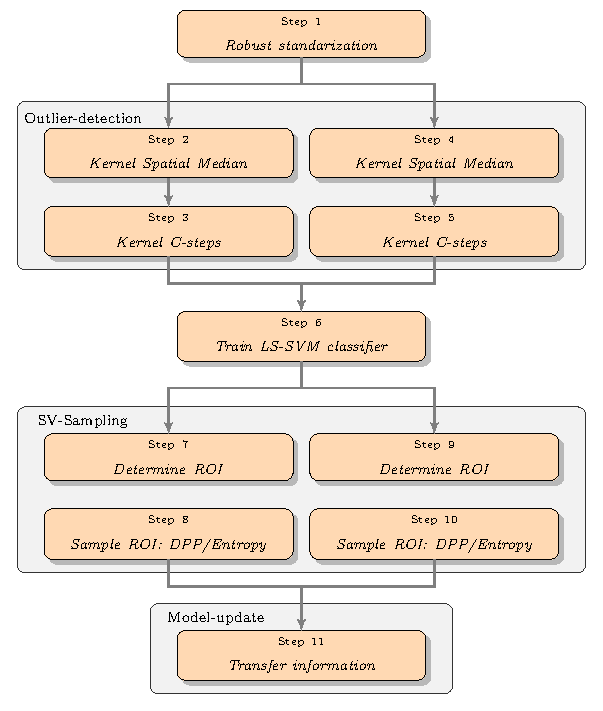
\includegraphics[width=0.8\linewidth]{flow/gabstract.pdf}
		\caption{Topological order of the LS-SVM pruning method. First, an outlier detection algorithm is used to extract regular observations; These samples are then used to build a classic LS-SVM model. As the classifier solution lacks sparsity, it is subjected to a sampling algorithm to extract support vectors. Finally, the trained model is converted to a sparse LS-SVM model by an information transfer step.  The outlier detection and landmark selection is done on each class separately which results in a parallel pipeline topology.} 
		\label{fig:pipeline}
	\end{figure}
%	@Iwein: even duidelijk uitleggen wat de definities zijn, welke subsets (en welke benaming) we gebruiken, consistent door de paper. 
%	\begin{enumerate}
%		\item Outlier vrije SV-candidates of REGULIERE OBSERVATIELIJST = h-subset resultaat, na reweighting, placed back in the original positions for both data subsets.
%		\item REGULIERE OBSERVATIELIJST: ROI bepaling geeft nieuwe lijst B: gepruned REGULIERE OBSERVATIELIJST.
%		\item geprunde REGULIERE OBSERVATIELIJST: DPP sampling geeft de SV lijst. 
%		\item Info transfer van vrije SV-candidates naar de SV lijst.
%	\end{enumerate}
%	
%	\begin{enumerate}
%		\item Outlier detection by kernel Csteps.
%		\item Train the robust LS-SVM by solving the system of equations.
%		\item Determine a region of interest (ROI), which is a reduction of the original dataset, that consist of points close to the decision boundary. This subset represent potential good support vector values.
%		\item Reduce the ROI even more by sampling the desired amount of support vector values using a method that promotes diversity:
%		\begin{enumerate}
%			\item Entropy
%			\item DPP
%		\end{enumerate}
%		\item Transfer the information of non-selected support vectors to selected ones.
%	\end{enumerate} 
	
	%\newpage
	\subsection{Outlier detection in kernel feature space}
	 Modern multivariate robust statistical methods are frequently based on the Minimum Covariance Determinant (MCD) method, first introduced in~\cite{rousseeuw1985multivariate}. This Mahalanobis distance based estimator can withstand a substantial amount of trainingset contamination (up to 50\%), and is nowadays (also) employed as refinement step. Robust two-step mechanisms (initial estimation $\rightarrow$ refinement) inherit the robustness of the MCD, but offers an improved statistical efficiency [see e.g.~\cite{hubert2015dets}]. Deterministic variants and well know PCA-based applications are described in \cite{hubert2012deterministic} and \cite{hubert2005robpca} respectively. \\
	
	Given a trainingset $X$ of $n$ observations in $p$ dimensions, the MCD-objective is to find the $h$ observations whose sample covariance matrix has the lowest possible determinant, where the amount of regular observations $h < n$ is specified before the algorithm starts. The MCD-estimate of location $c_h$ is then the average of these $h$ points (the $h$-subset), whereas the scatter estimate is a multiple of their covariance matrix $\hat{\Sigma}_{h}$. 
	
	In order to find the MCD-estimate, the FastMCD-algorithm~\cite{rousseeuw1999fast} uses so-called concentration steps (C-steps). Based on its robustness properties, simplicity and proven convergence, we propose to modify the C-step algorithm so that it can work in kernel feature space. This, in turn, allows the detection of \textit{non-linear} outliers: a noteworthy difference compared to off-the-shelve robust statistical algorithms as normality is frequently assumed. \\
	
	To enable the C-steps methodology in feature space $\mathcal{H}$, we integrate the mapping function $\phi(.)$ in the required algorithm formula's: 
	\begin{equation}
	\label{eq:center}
	c_h = \frac{1}{h} \sum_{i=1}^{h}\phi(x_i).
	\end{equation}
	Likewise, the Mahalanobis distance in $\mathcal{H}$ is defined as:
	\begin{equation}
	\label{eq:smd}
	||\phi(x) - c_h||^2_{\Sigma_h} = (\phi(x) - c_h) \Sigma^{-1}_h (\phi(x) - c_h).
	\end{equation}
	Where the biased covariance matrix of the $h$-subset is calculated as:
	\begin{equation}
	\Sigma_h = \frac{1}{h} \sum_{i=1}^{h} (\phi(x_i) - c_h) (\phi(x_i) - c_h)^T.
	\label{eq:sigma}
	\end{equation}
	As we do not explicit know the mapping function $\phi(.)$, equation \eqref{eq:smd} cannot be calculated, a problem circumvented by the eigendecomposition of the covariance matrix:
	\begin{equation}
	\Sigma_h = V^T D V.
	\end{equation}
	Where $V$ is the matrix of eigenvectors $v^k$ and $D$ resembles the diagonal matrix of eigenvalues $\lambda^k$ for $k=1,2, \dots, h$. The relation between eigenvalues and eigenvectors follows the identity:
	\begin{equation}
	\label{eq:eigenrelation}
	\Sigma_h v^k = \lambda^k v^k.
	\end{equation} 
	From the definition of equation \eqref{eq:sigma}, it can be seen that each eigenvector is a linear combination of the observations $\phi(x_i)$ in kernel feature space:
	\begin{equation}
	v^k = \sum_{1}^{n} \alpha_i^k ( \phi(x_i) - c_n). 
	\end{equation}
	If we substitute the above in equation \eqref{eq:eigenrelation}, it follows that:
	\begin{equation}
	n \lambda^k \alpha^k = \tilde{K} \alpha^k.
	\end{equation}
	Here, $\tilde{K}$ denotes the symmetric kernel matrix of $h$ rows, centered in $\mathcal{H}$. The weights $\alpha$ are determined by solving the eigendecomposition problem. \\
	By refactoring $\Sigma^{-1}$ as $V^T D^{-1/2} D^{-1/2} V$ and exploiting reductant operations in the Mahalanobis distance formula, Nader et al.~\cite{nader2014mahalanobis} show that equation~\eqref{eq:smd} can be calculated in $\mathcal{H}$ as:
	\begin{equation}
	\label{eq:Mahal}
	||\phi(x) - c_n||^2_{\Sigma} = \sum_{k=1}^{n} (\lambda^k)^{-1} \big( \sum_{k=1}^{n} \alpha^k \tilde{k}(x_i, x) \big)^2.
	\end{equation}	
		
Finally, the centered kernel matrix $\tilde{K}$ is calculated as~\cite{scholkopf1998nonlinear}:
	\begin{align}
	\label{eq:centerKh}
	\tilde{K}_{ij} &= \Big(\phi(x_i) - \frac{1}{n}\sum_{m=1}^n\phi(x_m)\Big) \cdot \Big(\phi(x_j) - \frac{1}{n}\sum_{k=1}^n\phi(x_k)\Big) \\
	&= K_{ij} - \frac{1}{n}\sum_{m=1}^n K_{mj} - \frac{1}{n}\sum_{k=1}^n K_{ik} + \frac{1}{n^2}\sum_{m=1}^n\sum_{k=1}^n K_{mk} \\
	&= \Big(K - 1_n K - K1_n + 1_n K1_n\Big)_{ij},
	\end{align}
	where $ \tilde{K} \in \mathbb{R}^{n \times n}$ and $1_n \in \mathbb{R}^{n\times n}$ with all entries set to $1/n$. 
	The centering of the kernel matrix of $t$ observations, given the original trainingset follows a similar derivation:
	\begin{align}
	\label{eq:centerKt}
	\tilde{K_t} &= K_t - 1_t K - K_t 1_n + 1_t K1_n,
	\end{align}
	with kernel matrix $ \tilde{K}_t \in \mathbb{R}^{t \times n}$ and the matrix $1_t \in \mathbb{R}^{t \times n}$ with all entries set to $1/n$. Using the methods we have discussed so far, our outlier detection algorithm is as follows. \\
	
	Start with the robust standardization of each observation: 
	
	\begin{equation}
		z_i = \frac{(x_i - \hat{\mu}_{mcd})}{\hat{\sigma}_{mcd}} ,
	\end{equation}
	
	where $\hat{\mu}_{mcd}$ and $\hat{\sigma}_{mcd}$ are the univariate location and scale estimations of the univariate MCD~\cite{rousseeuw1999fast}, estimated on the entire dataset. this procedure reduces the impact of different feature scales. Next, the standardized dataset is split in two subsets according to its class label $y \in \{+1, -1\}$ and our proposed  procedure is applied (per subset) to derive at an outlier free support vector candidate set, as follows:
	
	\begin{enumerate}
		\item[]\textbf{Algorithm 1: Outlier detection using kernel c-steps}
		\item Calculate the spatial median in $\mathcal{H}$, as introduced in~\cite{debruyne2010detecting}. The spatial median can be written as a linear combination of the feature vectors. Denote $\gamma = (\gamma_1, \dots, \gamma_n)^T$ the vector of coefficients, where  $\sum_{i=1}^{n} \phi(x_i) \gamma_i$ equals the spatial median in feature space. Initialise $\gamma = (1/n, 1/n, \dots)$ and recursively compute the normalized coefficients $\gamma = w / \sum_{i=1}^{n}w_i$, where $w_i$ for the observation with index $i$ is calculated as:
		\begin{equation}
		w_i = \frac{1}{\sqrt{ K_{i,i} - 2 \gamma^T K_{., i} + \gamma^T K \gamma}}.
		\end{equation}
		Ten iterations are usually enough to obtain a good approximation.	
		\item  Calculate the Euclidean distance for each observation to the spatial median:
		\begin{align}
		d_i &= || \phi(x_i) - \sum_{j=1}^N \gamma_j \phi(x_j)||^2 \\
		&= || \phi(x_i)||^2 + || \sum_{j=1}^N \gamma_j \phi(x_j)||^2 - 2 <\phi(x_i),\sum_{j=1}^N \gamma_j \phi(x_j)> \\
		&= K(x_i,x_i) + \sum_{j=1}^N \sum_{k=1}^N \gamma_j \gamma_k K(x_j,x_k) - 2 \sum_{j=1}^N\gamma_j K(x_i,x_j).
		\end{align}
		\item 	Sort these distances in ascending order. Define the initial $h$-subset by the $h_{init}$ observations with the lowest distance.	
		
		\item Apply kernel C-step for a fixed amount of iterations as follows:
		
		\begin{enumerate}
			\item Calculate the kernel matrix $K_h$ for the given $h$-subset of observations.
			\item Center $K_h$ in $\mathcal{H}$ by equation \ref{eq:centerKh}, obtaining $\tilde{K}_h$
			\item Perform the singular value decomposition on $\tilde{K}_h$ to obtain the eigenvectors $\alpha$ and eigenvalue vector $L_d$.
			\item Normalize each eigenvector $\alpha^k$ by its corresponding eigenvalue $\lambda_k$:
			\begin{equation}
			||\alpha^k|| = \frac{1}{n\lambda_k}, \mathrm{for \enskip all \enskip components \enskip}k.
			\end{equation}
			\item Calculate the kernel matrix for the given $h$-subset of observations in $n$ features.
			\item Center the kernel matrix by equation~\eqref{eq:centerKt} and obtain the Mahalanobis distances with equation~\eqref{eq:Mahal} or, expressed in vector notation:
			\begin{equation}
				d^2  = (\tilde{K_t}\alpha)^{\circ 2}\lambda^{-1},
			\end{equation}
			where  $d^2 \in \mathbb{R}^{n \times 1}$, $ \tilde{K_t} \in \mathbb{R}^{t \times n}$, $\lambda^{-1} = [\lambda_1^{-1} ,...,\lambda_k^{-1}]^\mathrm{T} \in \mathbb{R}^{k \times 1}$ , $\alpha \in \mathbb{R}^{n \times k}$ and $^{\circ 2}$ the 
			element-wise square.
			\item Sort the distance vector $d^2$ in ascending order and redefine the $h$-subset as the $h$ observations with smallest distance.
			\item If the new $h$-subset is equal to the previous one, exit the C-step loop.
		\end{enumerate}
		
		\item  If the $h$-subset size is lower then $h_{end}$, increase the $h$-subset size by (say) 5\% and go back to step 4. 
		\item  Determine the final support vector candidate mask. Assign a binary weight to each observation $i$:
		\begin{equation}
			w(d^2)  =
			\begin{cases}
			1       & \quad \text{if } d^2 \leq c \\
			0  & \quad \text{if } d^2 >c
			\end{cases}
		\end{equation}
		where $c$ is a threshold which we choose here as $c = max(\chi_p^2(0.975), max(d_h^2) )$, with $d_h^2$ the distance vector of the observations in the $h$-subset. 
%		\begin{equation}
%		w_i =
%		\begin{cases}
%		1, & \text{if}\ rd^2(i) \leq max(\chi^2_{0.975, p}, rd^2(h\mathrm{-subset})) \\
%		0, & \text{otherwise}
%		\end{cases}
%		\end{equation}
	\end{enumerate}
	
	Finally, the weights $w$ are then used to train a weighted LS-SVM, where only the points with a weight equal to 1 are used in training the model. The algorithm workings are visualised in Figure \ref{fig:C-step}, where it can be seen that the initial estimate converges to the (linear and non-linear) outlier free observation subset.
	
	
	\begin{figure}[!htb]
		\centering
		\begin{subfigure}[b]{0.40\linewidth}
			\centering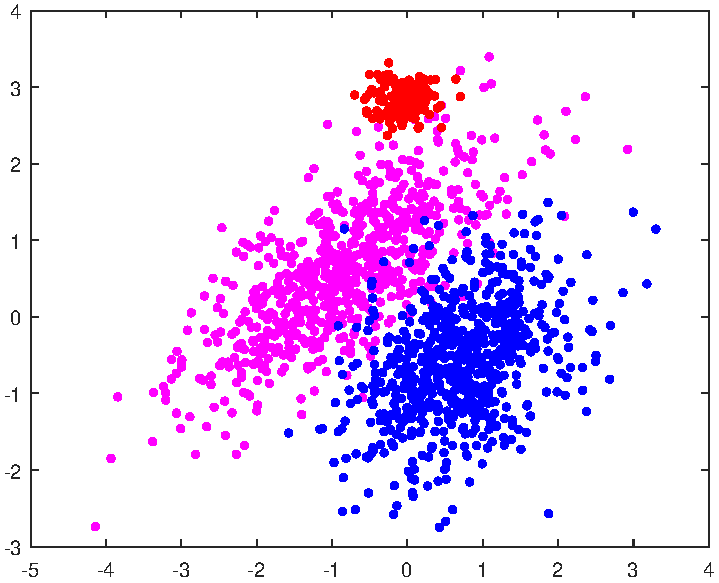
\includegraphics[width=1\linewidth]{figures/kcstep/nddatamodel.pdf}
			\caption{\label{fig:dmodel1}} 
		\end{subfigure}
		\begin{subfigure}[b]{0.40\linewidth}
		\centering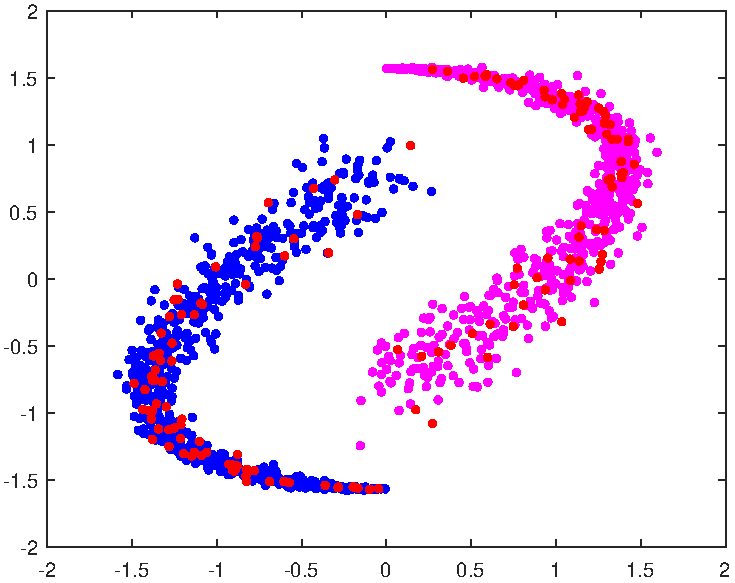
\includegraphics[width=1\linewidth]{figures/kcstep/yydatamodel.pdf}
		\caption{\label{fig:spatialmedc1}}
		\end{subfigure} \\

		\begin{subfigure}[b]{0.40\linewidth}
			\centering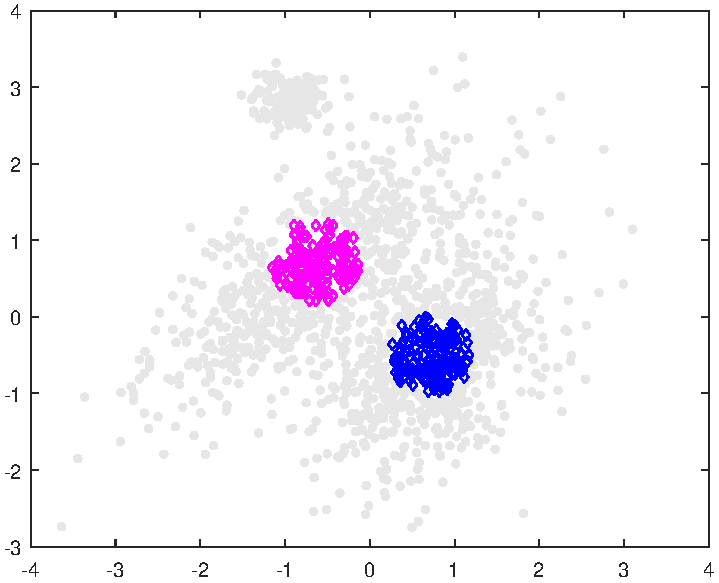
\includegraphics[width=1\linewidth]{figures/normdatamodel_sm.pdf}
			\caption{\label{fig:dmodel2}} 
		\end{subfigure} 
		\begin{subfigure}[b]{0.40\linewidth}
			\centering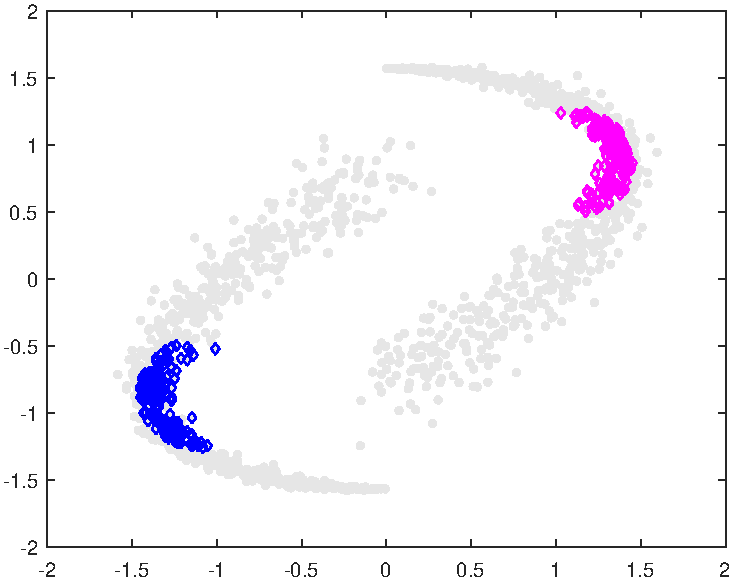
\includegraphics[width=1\linewidth]{figures/yydatamodel_sm.pdf}
			\caption{\label{fig:spatialmedc2}}
		\end{subfigure} \\
		
		\begin{subfigure}[b]{0.40\linewidth}
			\centering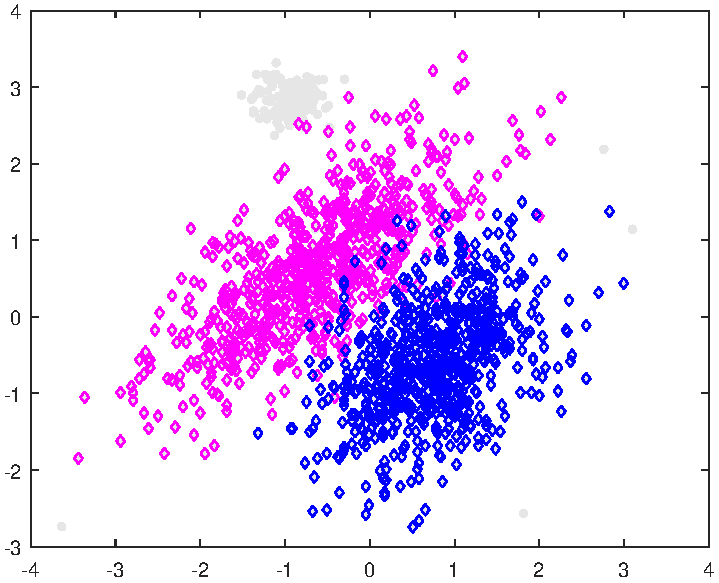
\includegraphics[width=1\linewidth]{figures/normdatamodel_kc.pdf}
			\caption{\label{fig:kcstepc1}}
		\end{subfigure}
		\begin{subfigure}[b]{0.40\linewidth}
			\centering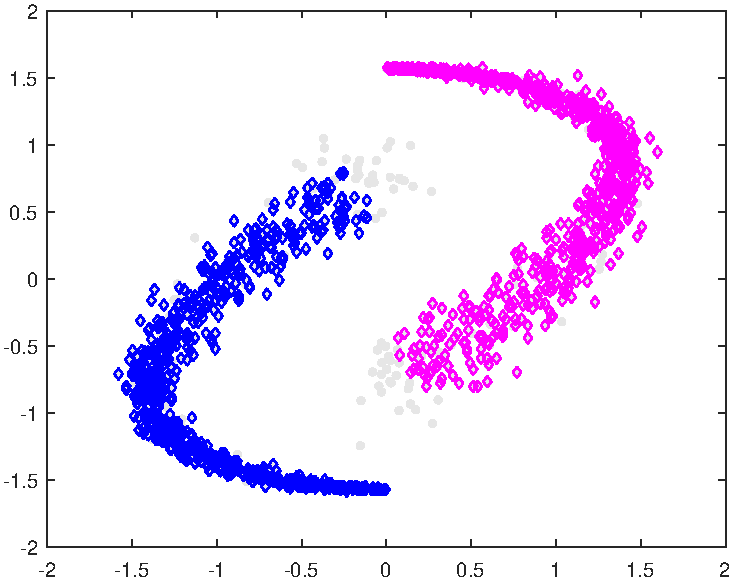
\includegraphics[width=1\linewidth]{figures/yydatamodel_kc.pdf}
			\caption{\label{fig:kcstepc2}}
		\end{subfigure}
		\caption{
			Figure \subref{fig:dmodel1} depicts a normal distributed, binary classification problem. A linear kernel will be used in the outlier detection of this dataset. Figure \subref{fig:dmodel2} shows a non-linear classification problem, where an RBF kernel with bandwidth $\sigma = 0.5$ is used.  Both classes (blue, green) contain $10\%$ outliers from, shown in red. After splitting the dataset by their class labels, the $h_ {init}$ closest points from the spatial median are used as initial subsets for the C-step algorithm [STEP 3], depicted in green for the first class of both datamodels (Figures \subref{fig:spatialmedc1}, \subref{fig:spatialmedc2}). After iterative kernel C-steps, we obtain the re-weighted results  [STEP 6], shown in Figures \subref{fig:kcstepc1} and \subref{fig:kcstepc2}. Support vectors are then determined from the detected regular observation list by a landmark selection algorithm (section \ref{sec:Sparseness}).}
		\label{fig:C-step}
	\end{figure}
	
	
	%\newpage
	\FloatBarrier
	
	\subsection{Imposing sparseness: support vector section methodology}
	\label{sec:Sparseness}
	
%	\subsection{}
	
	%Pruning implies that prediction formula (REF TO EQUATION) should be partitioned in a \textit{relevant} (the support vectors or landmark points, found by the pruning algorithm) - and \textit{irrelevant} part.  
	%An overview of existing pruning methods can be found in Hoegaerts et al. \cite{hoegaerts2004comparison}. 
	The next step in the algorithm is introducing sparseness by pruning the previously trained robust LS-SVM.
	A first LS-SVM pruning approach was suggest by Suykens et al.~\cite{suykens2000sparse}, where  sparseness is imposed by pruning support values from the sorted support value spectrum resulting from the solution to the linear system.  The motivation comes from the fact that LS-SVM support values are proportional to the errors at datapoints. Thus omitting the points that contribute least to the training error. The values with a high $|\alpha_k|$ reside close to the decision boundary and are thus important to classify correctly. 
	
	However blindly taking the points with largest support value spectrum could lead to sub-optimal results. Firstly, when outliers are present, you want to be certain that these are not chosen. Secondly, points are chosen independently towards each other. This results in clumping of landmarks. The first problem is addressed by running a kernelized minimum covariance determinant, which detects and omits potential outliers.  \\
	
	The second problem is solved by introducing a subset for each class \newline $y \in \{+1,-1\}$ called the "region of interest" (ROI), which consist of points close to the decision boundary. Determining the ROI is done for each class and consists out of two steps:
	\begin{enumerate}
		\item[]\textbf{Algorithm 2: Determining the ROI}
		\item Determine the subset which consists of all points belonging to the class and are not considered outliers by the kernel MCD procedure.
		\item Reduce the subset by selecting the points where the sign of $\alpha_i$ is equal to sign of the currently analyzing class.
		\item The subset is further reduced by selecting the points that satisfy:
		\begin{equation}
			|\alpha_i| \geq \mathrm{median}(|\alpha|), \mathrm{for} \enskip i = 1,...,j
		\end{equation}
		 where $\alpha = [\,|\alpha_1|,...,|\alpha_j|\,]^{\mathrm{T}}$ and $\alpha_i$ the support value of points in the subset of step 2 with cardinality $j$.
	\end{enumerate}

	\begin{figure}[!htb]
	\centering
	\begin{subfigure}[b]{0.40\linewidth}
		\centering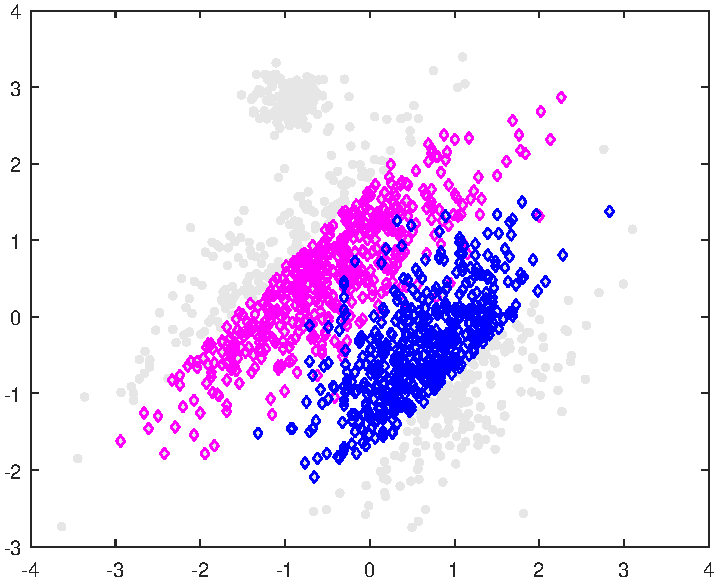
\includegraphics[width=1\linewidth]{figures/normdatamodel_landm1.pdf}
		\caption{\label{fig:sparse1}} 
	\end{subfigure}
	\begin{subfigure}[b]{0.40\linewidth}
		\centering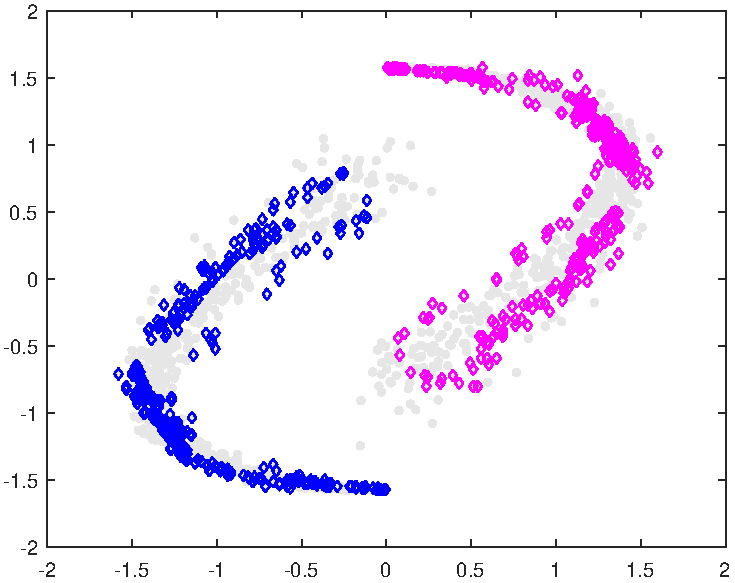
\includegraphics[width=1\linewidth]{figures/yydatamodel_landm1.pdf}
		\caption{\label{fig:sparse2}}
	\end{subfigure} \\
	
	\begin{subfigure}[b]{0.40\linewidth}
		\centering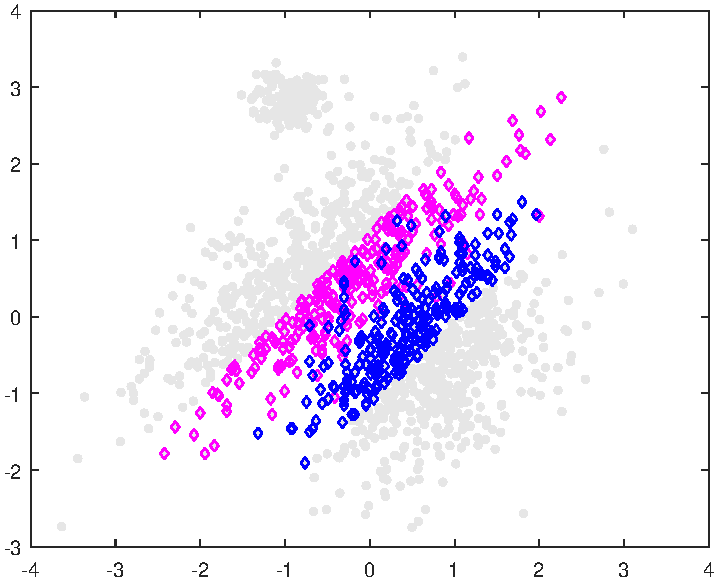
\includegraphics[width=1\linewidth]{figures/normdatamodel_landm2.pdf}
		\caption{\label{fig:ROI1}} 
	\end{subfigure} 
	\begin{subfigure}[b]{0.40\linewidth}
		\centering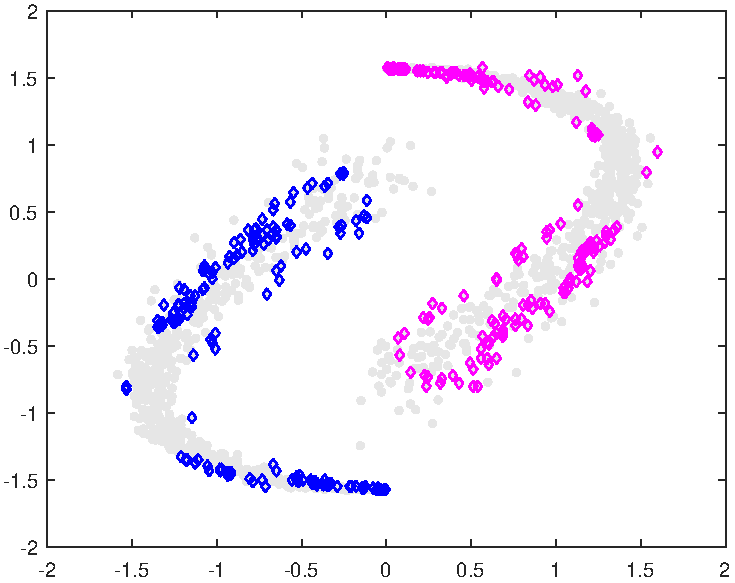
\includegraphics[width=1\linewidth]{figures/yydatamodel_landm2.pdf}
		\caption{\label{fig:ROI2}}
	\end{subfigure} \\
	
	\begin{subfigure}[b]{0.40\linewidth}
		\centering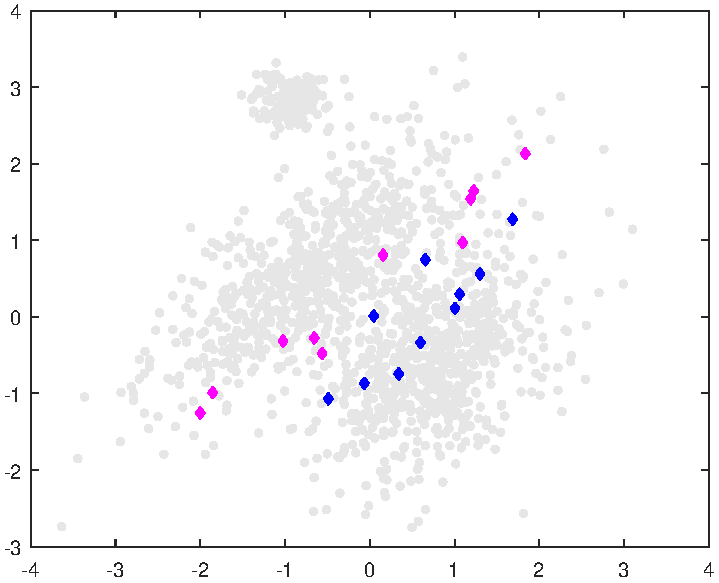
\includegraphics[width=1\linewidth]{figures/normdatamodel_landm3.pdf}
		\caption{\label{fig:DPP1}}
	\end{subfigure}
	\begin{subfigure}[b]{0.40\linewidth}
		\centering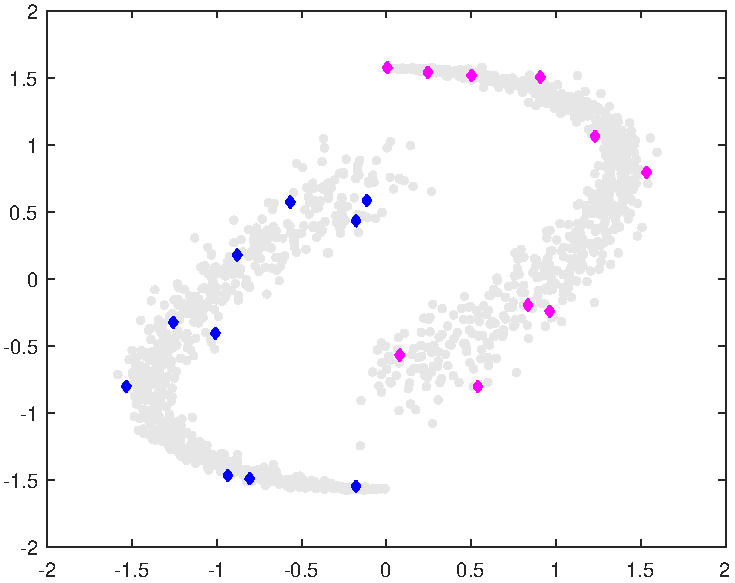
\includegraphics[width=1\linewidth]{figures/yydatamodel_landm3.pdf}
		\caption{\label{fig:DPP2}}
	\end{subfigure}
	\caption{An example of the sparsification procedure where the same datasets as in Figure \ref{fig:C-step} are analysed. Figures \subref{fig:sparse1} and \subref{fig:sparse2} show step 2 of the ROI algorithm, where only points that have an equal sign to the corresponding class are selected. The subset if reduced even further by selecting points with the largest contribution to the decision boundary. This corresponds to step 3 of the ROI algorithm and is visible on Figures \subref{fig:ROI1} and \subref{fig:ROI2}. The final step is sampling diverse points out of the ROI. Figures \subref{fig:DPP1} and \subref{fig:DPP2} show the result of this procedure, where the ROI is nicely approximated and no clumping effect is visible.}
	\label{fig:sparsensses}
	\end{figure}

	In contrast to the proposed pruning strategy by Suykens et al.~\cite{suykens2000sparse}, the sign of alphas is taken in consideration when determining the ROI (step 2). Potential landmark points are now points with large importance and that predict the right class. This is easily seen from the prediction equation \eqref{eq:classification}, where the contribution of a training point in the prediction a test point $x_t$ towards class $y \in \{+1,-1\}$ is proportional to $y \, \mu_i$, where $\mu_i = \alpha_i \, y_i$. Figure \ref{fig:C-step} confirms this behavior, where the ROI represents a subset with points important for the decision boundary for every class. Using a sampling algorithm that promotes diversity, $l$ landmark points are selected for every class to represent the ROI. Due to the diversity, no clumping is possible.
	
	\subsubsection{Entropy}
	Selection of the landmark points is based on quadratic Renyi entropy~\cite{girolami2002orthogonal} and the fixed size LS-SVM~\cite{suykens2002least}. The landmarks points are chosen to maximize the quadratic Renyi Entropy:
	\begin{equation}
	\label{eq:Entropy1}
	H_R = -\mathrm{log}\int p(x)^2 dx.
	\end{equation}
	The quadratic Renyi Entropy is approximated by the following equation\cite{girolami2002orthogonal}:
	\begin{equation}
	\label{eq:Entropy2}
	\int \hat{p}(x)^2dx = \frac{1}{N^2} 1_v^\mathrm{T}\Omega 1_v,
	\end{equation}
	where $1_v = [1;1;...;1]$ and a normalized kernel is assumed with respect to density estimation. Entropy quantifies the diversity or randomness of a system, which is essential to select landmark points such that no clumping is possible . In the fixed-size LS-SVM approach, one chooses a fixed working set of size $M$ which is initialized randomly. Afterwards, random points are swapped in and out. If the entropy increases, the swapped point is accepted, otherwise the original subset is kept. This process continues until the change in entropy is small or a fixed number of iterations is reached. 
	
	In contrast to the original fixed-size LS-SVM formulation, which is used to find a representative subset for the Nystr\"{o}m approximation \cite{suykens2002least}. We propose to first determine to ROI, which includes the points that have the highest contribution to the robust LS-SVM model. On this reduced dataset, the fixed-size LS-SVM algorithm is used to select the $l$ landmark points. This ensures that the ROI is well approximated and there is no clumping effect present. The downsides of the entropy criteria are that a relatively large number of iterations are necessary to get a diversified selection, secondly only the Gaussian kernel can be used~\cite{girolami2002orthogonal}.
	
	
%	\begin{remark}
%		It is important to first omit outliers, before continuing with the entropy procedure. Large contributions to the entropy will come from elements that have little or no structure~\cite{girolami2002orthogonal}.
%	\end{remark}
	
	Given the ROI of candidate support vectors for a class $y \in \{+1,-1\}$, the entropy based selection algorithm is repeated for every class~\cite{suykens2002least}:
	\begin{enumerate}
		\item[]\textbf{Algorithm 3: Entropy based landmark selection}
		\item Choose a working set of size $l$ by randomly selection support vector out of the ROI.
		\item Randomly select a point out of the ROI and replace it by a random point in the working set.
		\item Calculate the quadratic Renyi entropy for the new working set using equations \eqref{eq:Entropy1} and \eqref{eq:Entropy2}.
		\item If the entropy increases, keep the swapped point, otherwise return to the original working set.
		\item Stop if the change in entropy is small or a maximum number of iterations is reached. Otherwise go back to step 2.
	\end{enumerate}
		

	\subsubsection{Determinantal point process}
	Selection of landmark points is based on determinantal point processes (DPPs)~\cite{kulesza2012determinantal}. DPPs are particularly interesting for set selection problems where diversity is preferred. A point process $\mathcal{P}$ on a ground set $\mathcal{Y} = {1,2,...,N}$ is a probability measure over point patterns of $\mathcal{C}$ , which are finite subsets of $\mathcal{Y}$. When $\mathcal{C}$ is a random subset, drawn according to the DPP $\mathcal{P}$, we have:
	\begin{equation}
	\label{eq:origDPP}
	\mathcal{P}(C \subseteq \mathcal{Y}) = \mathrm{det}(K_{\mathcal{C}}),
	\end{equation}
	where $K \preceq I$ is a positive symmetric semidefinite matrix with all eigenvalues smaller then or equal to 1, containing the index elements of $\mathcal{Y}$. $K_{\mathcal{C}} = [K_{i,j}]_{i,j \in \mathcal{C}}$ contains the selected rows and columns of $K$ and $\mathrm{det}(K_{\emptyset}) = 1$. From equation \eqref{eq:origDPP} follows:
	\begin{align}
	\mathcal{P}(i \in \mathcal{Y}) &= K_{i,i} \\
	\mathcal{P}(i,j \in \mathcal{Y}) &= K_{i,i}K_{j,j} - K_{i,j}K_{j,i}\\
	\label{eq:KDPP}
	&= \mathcal{P}(i \in \mathcal{Y})\mathcal{P}(j \in \mathcal{Y}) - K_{i,j}^2.
	\end{align}
	The diagonal elements of the kernel matrix give the marginal probability of inclusion for individual elements of $\mathcal{Y}$, whereas the off-diagonal elements determine the (anti-)correlation between pairs of elements. Thus for large values of $K_{i,j}$, or a high similarity, points are unlikely the appear together. DPP's are probabilistic models with global, negative correlations with respect to a similarity measure, this ensures diversity.
	
	In our case, we would like to build a DPP based on the kernel matrix $K$, which is done using L-ensembles~\cite{kulesza2012determinantal}. The probability of observing a subset $C \subseteq \mathcal{Y}$ is now equal to:
	\begin{equation}
	\mathrm{Pr}(\mathcal{C}) = \frac{\mathrm{det}(K_{\mathcal{C}})}{\mathrm{det}(K + I)},
	\end{equation}
	where $I$ is the identity matrix, and $K$ a positive semidefinite matrix  indexed by the elements of $\mathcal{Y}$. In contrast to equation \eqref{eq:origDPP}, $K$ only has to be positive semidefinite, while the eigenvalues previously where bounded above. Sampling a DPP is done in two phases~\cite{kulesza2012determinantal}. In the first phase, a subset of the eigenvectors $V$ of the kernel matrix $K$ is selected at random, where the probability of selecting each eigenvector depends on its associated eigenvalue. In the second phase, a sample $Y$ is produced based on the selected vectors. Note that on each iteration of the second loop, the cardinality of $Y$ increases by one and the dimension of $ V$ is reduced by one. When conditioning on a fixed cardinality $k = |\mathcal{C}|$, one gets the k-DPP~\cite{kulesza2011k}. 	
	
	The landmark selection algorithm consists of the following steps:
	We propose to first determine the ROI, which includes the points that have the highest contribution to the robust LS-SVM model. On this reduced dataset, a $k$-DPP~\cite{kulesza2011k}, where $k = l$, is used to sample the $l$ landmark points. This ensures that the ROI is well approximated and there is no clumping effect present. 
%	
%	\begin{remark}
%		It is important to first omit outliers, before continuing with the k-DPP sampling. In order to promote diversity, points that have a high similarity have a low chance of being sampled together (see equation \eqref{eq:KDPP}). Consequently outliers, that have a low similarity to any other point in the dataset, have a high chance of being sampled.
%	\end{remark}
	
Given the ROI of candidate support vectors for a class $y \in \{+1,-1\}$, the k-DPP selection algorithm is repeated for every class to select $l$ landmark points~\cite{kulesza2011k}: 
\begin{enumerate}
	\item[]\textbf{Algorithm 4: k-DPP based landmark selection}
	\item Calculate the eigenvector/value pairs $\{(v_r,\lambda_r)\}$ from the L-ensemble matrix $L = K_{R}(I - K_{R} )^{-1}$, where $K_{R} \in \mathbb{R}^{N_{R} \times N_{R}} $ is the kernel matrix containing the points in the ROI.
	\item Iterate over all components of the eigenvector/value pairs and include the component $r$ if:
	\begin{equation}
		u \sim U[0, 1] < \lambda_r \frac{e_{k-1}^{r-1}}{e_k^r},
	\end{equation}
	  where $k$ is number of components selected so far, iterator $r = N_{R},...,1$  and $k$ elementary polynomial $e_k^r = \sum_{\substack{J \subseteq \{1,...,r\}\} \\ |J| = k}}\prod_{n \in J} \lambda_n$ . Continue to the next step if you have selected $l$ components. The matrix $V$ is now equal to the eigenvectors of included components. 
	\item Select a landmark point $x_i$ from ROI with probability:
	\begin{equation}
		\mathrm{Pr}(x_i) = \frac{1}{|V|} \sum_{v \in V} (v^\mathrm{T} e_i)^2.
	\end{equation} 
	The vector $e_i$ is the $i$th standard basis, which is all zeros except for a one
	in the $i$th position.
	\item Recalculate $V \leftarrow V_\perp$, an orthonormal basis for the subspace of $V$ orthogonal to $e_i$. Afterwards go back to step 3 until $l$ landmark points are selected.
\end{enumerate}

%	\begin{remark}
%		It is important to first omit outliers, before continuing with the entropy procedure. Large contributions to the entropy will come from elements that have little or no structure~\cite{girolami2002orthogonal}.
%		It is important to first omit outliers, before continuing with the k-DPP sampling. In order to promote diversity, points that have a high similarity have a low chance of being sampled together (see equation \eqref{eq:KDPP}). Consequently outliers, that have a low similarity to any other point in the dataset, have a high chance of being sampled.\\	
%		As the outlier detection and landmark selection is done on each class separately. The proposed method is easily applicable in a multi-class classification setting. 
%	\end{remark}
	
	\subsection{Information transfer}
	The information contained in the not selected support vectors can then be transferred to the selected support vectors, an idea originally introduced in~\cite{tao2009fast}. Starting from equation \eqref{eq:classification} for the outlierfree dataset, we get in matrix notation:
	\begin{equation}
\hat{y} = \mathrm{sign}(K\beta  + b 1),
	\end{equation}
with $\hat{y} = [\hat{y}_1;...;\hat{y}_h]$ the prediction vector and $\beta = [\alpha_i y_i ,...,\alpha_i y_{h}]^\mathrm{T}$, where $h$ is the number of points in the outlierfree dataset.
We can partition this expression in the selected landmark part and non-selected support vectors:
	\begin{equation}
	\label{eq:twoparts}
\hat{y} = \mathrm{sign}(K_l\beta_l + K_{nl}\beta_{nl}  + b 1),
	\end{equation}
	where $K_l $ is the matrix whose columns are selected from $K$ using the landmark selection while the other columns of $K$ form matrix $K_{nl}$, and $\beta_l$ is a column vector whose elements are the multipliers corresponding to columns in $K_l $ while the other multipliers compose the vector $ \beta_{nl}$.
	Next, one transfers the information of $\beta_{nl} K_{nl}$ using the update $\Delta\beta$: 
	\begin{align}
	\Delta \beta K_l &= K_{nl} \beta_{nl}   \\
	\Delta \beta &= K^\dagger_l  K_{nl} \beta_{nl},
	\label{eq:deltaBeta}
	\end{align}
	where $\dagger$ is the Moore-Penrose inverse. We now have obtained an explicit expression for the update of our Lagrange multipliers:
	\begin{align}
	\label{eq:deltaBetaAdd}
	\hat{\beta}_l &=\beta_l + \Delta \beta.
	\end{align}	
 The classier prediction equation finally boils down to:
	\begin{equation}
	\label{eq:LastClass}
\hat{y}(x) = \mathrm{sign}\Big(\sum_{i=1}^{l} K(x, x_i)\hat{\beta}_i  + b\Big).	
	\end{equation}
	
Given the outlierfree dataset from algorithm 1, the trained LS-SVM model based on this outlierfree dataset and the selected support vectors based on algorithm 3, the information transfer is done in the following way: 
	\begin{enumerate}
		\item[]\textbf{Algorithm 5: Information transfer}
		\item Split the prediction equation for the training set in two parts containing the selected support vectors and non-selected support vectors (see equation~\eqref{eq:twoparts}).
		\item Determine the update for $\Delta \beta$ using equation \eqref{eq:deltaBeta}.
		\item Update the support vectors using formula~\eqref{eq:deltaBetaAdd} to get the final prediction equation~\eqref{eq:LastClass}.
	\end{enumerate}
	
	\subsection{Summary Rob-LSSVM} 
	To finalize this section, we summarize the steps of the proposed algorithm. The following procedure is applied on a contaminated dataset $\{x_i,y_i\}_{i=1}^N$, where $x_i \in \mathbb{R}^{p}$ denotes $i$-th input pattern and $y_i \in \{-1,1\}$ the $i$th label :
	
\begin{enumerate}
	\item[]\textbf{Final algorithm: Rob-LSSVM}
	\item Run Algorithm 1 (Outlier detection using kernel c-steps) on each class. This results is an outlierfree dataset $\{x_i,y_i\}_{i=1}^h$, where is the number of regular observations.
	\item Train an LS-SVM classfier on this outlierfree dataset, which gives the support vector values $\{\alpha_i\}_{i=1}^h$ and bias term $b$. 
	\item Based on the support vector values, determine the ROI for each class using Algorithm 2.
	\item Select the final support vector values or landmark points for each class using a diverse sampling procedure (Algorithm 3 or 4). This results in $l$ landmark points for each class.
	\item Transfer the information from the support vector values of not selected support vectors to the selected support vectors using algorithm 5. The result is the Rob-LSSVM classifier.
\end{enumerate}

The final solution for the toy-datasets is visible on Figure~\ref{fig:results}, where extreme sparsity and a robust classification is achieved.


	\begin{figure}[!htb]
		\centering
		\begin{subfigure}[b]{0.40\linewidth}
			\centering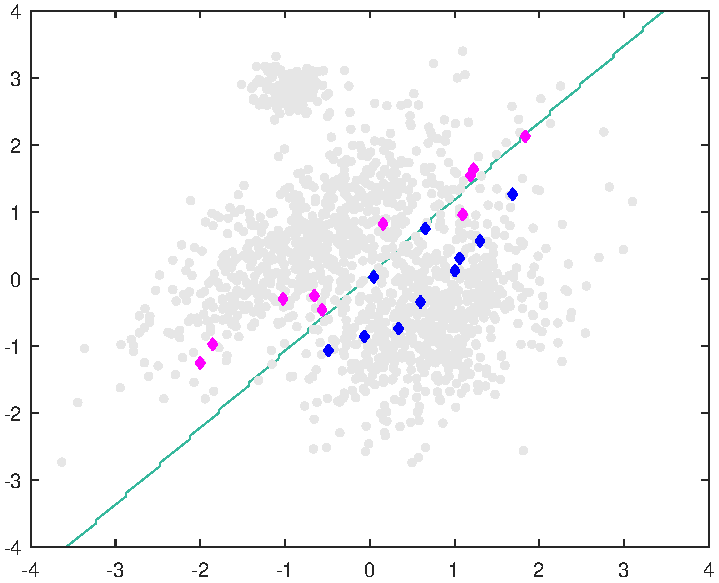
\includegraphics[width=1\linewidth]{figures/normdatamodel_hyperplane_robsvm.pdf}
			\caption{\label{fig:solRob1}} 
		\end{subfigure}
		\begin{subfigure}[b]{0.40\linewidth}
			\centering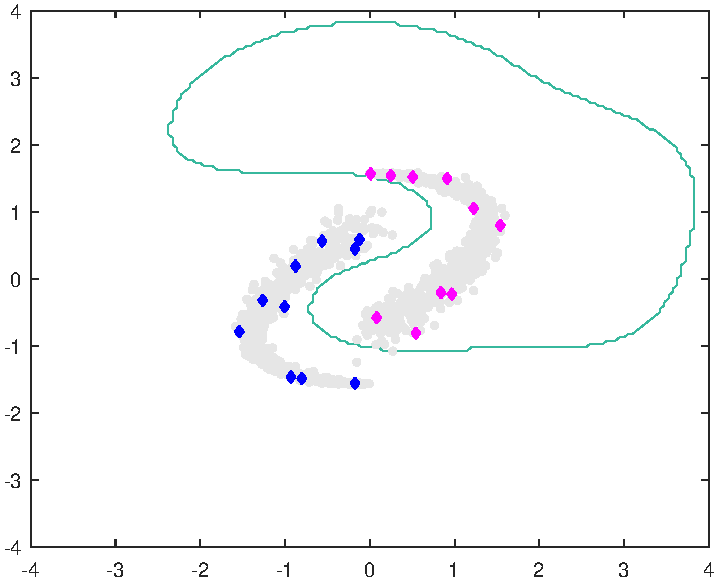
\includegraphics[width=1\linewidth]{figures/yydatamodel_hyperplane_robsvm.pdf}
			\caption{\label{fig:solRob2}}
		\end{subfigure} \\
		
		\begin{subfigure}[b]{0.40\linewidth}
			\centering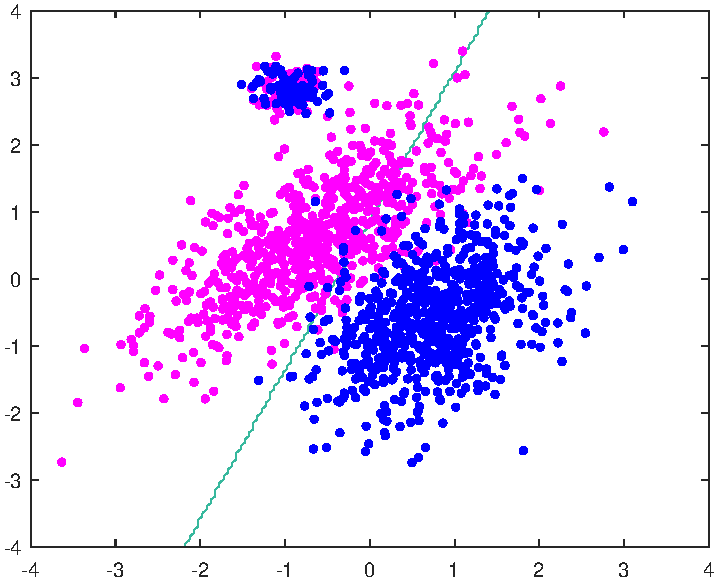
\includegraphics[width=1\linewidth]{figures/normdatamodel_hyperplane_lssvm}
			\caption{\label{fig:solNorm1}} 
		\end{subfigure} 
		\begin{subfigure}[b]{0.40\linewidth}
			\centering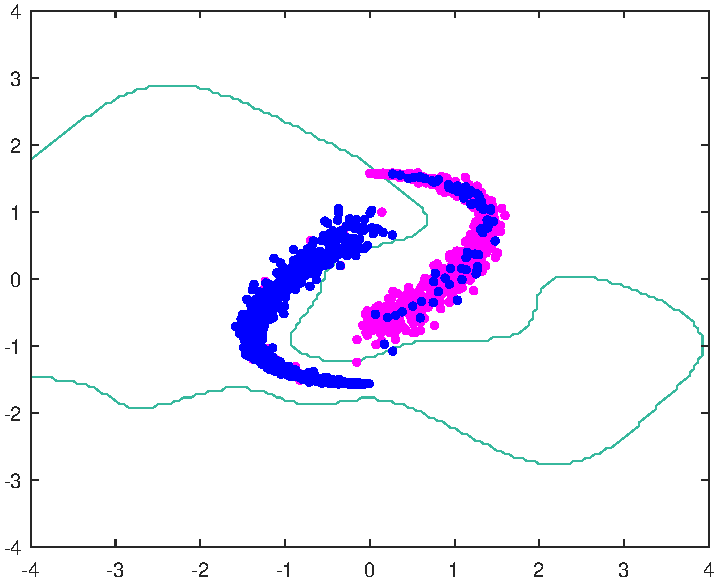
\includegraphics[width=1\linewidth]{figures/yydatamodel_hyperplane_lssvm.pdf}
			\caption{\label{fig:solNorm2}}
		\end{subfigure} 
		\caption{The final solution after applying RoS-LSSVM on the toy example is visible on Figures \subref{fig:solRob1} and \subref{fig:solRob2}. A robust classification is achieved, this while reducing the number of support vector to a bare minimum. The opposite effect is visible for the normal LS-SVM classification on Figure \subref{fig:solNorm1} and \subref{fig:solNorm2}. }
		\label{fig:results}
	\end{figure}
	
	\section{Experiments} 
	\label{sec:exp}
	\subsection{Simulation results} 
	
	\subsubsection{Linear example}
	
	Two Gaussians close, the reverse labels behind at large distance. See Robustified LS-SVM~\cite{debruyne2009robustified}
	
	\subsubsection{Non-Linear example}
	
	Yin-Yang, Two spiral dataset or Cross Dataset~\cite{yang2014robust}
	
	\subsubsection{UCI}
	
	Robust: Banana, Celveland heart, Glass, Heartstatlog, liver disorder, monk PIMA, ripley, Transfusion, Vehicle~\cite{yang2014robust}
	
	Robust + sparse: Splice, Pendigits (choose two digits 3 vs 4), Satimage (1 vs 6), USPS (1 vs 2), Mushrooms, Protein (1 vs 2).\cite{chen2018sparse}
	Outliers = 30 \% samples that where far away from decision hyperplane, then randomly sample 1/3 of them and flip labels. datasets are in https://www.csie.ntu.edu.tw/~cjlin/libsvmtools/datasets/ 
	
	Robust: Wine dataset + Linear, Glass, Biscuit Dough, Alon colon cancer, Hepatocellular carcinoma dataset~\cite{debruyne2009robustified}. However mostly linear
	
	\subsection{Industrial data results} 
	
	\section{Conclusions and future work}
	\label{sec:conc}
	
	We proposed a new, improved  LS-SVM model, coined RoS-LSSVM, inspired by the [WHAT, kernel C-steps, DPP, sampling, info transfer]-principle. We compared the performance of our prototype with other models by means of simulations for small, moderate and large UCI data sets. We found that our classifier model performed better than other models in terms of outlier robustness and classification accuracy. \\
	
	Further research should go to the extension of sparsity in the classifier training phase, as well as [???]. It would also be worthwhile to integrate an optimization routine to estimate the optimal $h$-subset size for a given problem, as no theoretical results can predict the contamination degree before the actual processing yet. 
	
	\section*{Acknowledgements}
	
	We thank Johan Speybrouck for providing us the industrial datasets, and Tim Wynants, Doug Reid for their feedback throughout this project. We also acknowledge the financial support of the VLAIO, grant HBC.2016.0208, for making this industrial research possible.
	
	%% The Appendices part is started with the command \appendix;
	%% appendix sections are then done as normal sections
	%% \appendix
	
	%% \section{}
	%% \label{}
	
	%% References
	%%
	%% Following citation commands can be used in the body text:
	%% Usage of \cite is as follows:
	%%   \cite{key}          ==>>  [#]
	%%   \cite[chap. 2]{key} ==>>  [#, chap. 2]
	%%   \citet{key}         ==>>  Author [#]
	
	%% References with bibTeX database:
	
	%\bibliographystyle{model1-num-names}
	\bibliographystyle{plain}
	\bibliography{sample}
	
	%% Authors are advised to submit their bibtex database files. They are
	%% requested to list a bibtex style file in the manuscript if they do
	%% not want to use model1-num-names.bst.
	
	%% References without bibTeX database:
	
	%\begin{thebibliography}{00}
	%
	%%% \bibitem must have the following form:
	%%%   \bibitem{key}...
	%%%
	%
	%
	%\end{thebibliography}
	
	
\end{document}

%%
%% End of file `elsarticle-template-1-num.tex'.